\documentclass[11pt,a4paper]{article}

\usepackage[utf8]{inputenc}
\usepackage[T1]{fontenc}
\usepackage{lmodern}
\usepackage[ngerman]{babel}
\usepackage{geometry}
\usepackage{graphicx}
\usepackage{booktabs}
\usepackage{amsmath}
\usepackage{amssymb}
\usepackage[colorlinks=true, allcolors=blue]{hyperref}
\geometry{a4paper, left=2.5cm, right=2.5cm, top=2.5cm, bottom=2.5cm}

\title{\textbf{Stoneforge RL --- Projektdokumentation}\\
\large Navigation in prozedural generierten Welten mit Reinforcement Learning:\\
Stand und Entwicklung}
\author{Florian Merlau \and Laurin}
\date{6. Juli 2026}

\begin{document}

\maketitle

\begin{abstract}
\noindent
Diese Dokumentation fasst den aktuellen Stand der Projektarbeit zusammen: ein
RL-Agent soll in prozedural generierten 2D-Welten (\emph{Stoneforge}) den Exit
finden und dabei auf unbekannte Seeds generalisieren. Der beste Agent
(RecurrentPPO mit LSTM, Curriculum-Training) erreicht \textbf{86\,\% Success
Rate} (stochastisch) auf dem Testset bzw.\ 68\,\% auf dem Holdout-Set und
übertrifft damit beide Zielkriterien ($\geq$70\,\% / $\geq$60\,\%). Dokumentiert
werden die Umgebung, die Methodik, die zentrale Ablation (MLP vs.\ LSTM), der
vollständige Entwicklungsverlauf von Projektbeginn bis heute (inkl.\ negativer
Ergebnisse und Root-Cause-Analysen, Quelle: Experiment-Changelog), die
Umgebungsrevision v11 vom 06.07.2026 sowie eine Performance-Analyse (CPU vs.\
Apple-GPU, Batch-Größe), die die Trainingszeit halbiert.
\end{abstract}

\section{Zielsetzung}

Gegenstand der Projektarbeit ist die Frage, ob ein Reinforcement-Learning-Agent
in prozedural generierten, nur teilweise beobachtbaren 2D-Welten robuste
Navigationsstrategien lernen kann, die auf unbekannte Welten (neue Seeds)
generalisieren --- statt einzelne Karten auswendig zu lernen
\cite{cobbe2020procgen, risi2020increasing}. Als Erfolgskriterien wurden vorab
definiert:

\begin{itemize}
  \item \textbf{Testset A} (Seeds 7000--7049): $\geq 70\,\%$ Success Rate,
  \item \textbf{Holdout B} (Seeds 8000--8049): $\geq 60\,\%$ Success Rate,
  \item pro Konfiguration mindestens 3 Trainingsläufe (Mittelwert $\pm$ Standardabweichung).
\end{itemize}

\section{Die Umgebung Stoneforge}

Stoneforge ist ein selbst entwickeltes, rundenbasiertes 2D-Spiel (C++-Kern,
Python-Anbindung über pybind11). Die Welt wird pro Seed deterministisch aus
Hash-Noise generiert (7 Biome, Chunks à $16{\times}16$ Tiles, theoretisch
unendlich); der Agent startet bei $(0,0)$ und muss den Exit erreichen.

\subsection{POMDP-Charakter}

Der Agent sieht nur einen lokalen $15{\times}15$-Ausschnitt der Welt sowie einen
\emph{Luftlinien}-Kompass zum Exit --- nicht den Weg. Wände, Sackgassen und
Umwege außerhalb des Sichtfensters sind unbekannt: Die Aufgabe ist ein
\emph{Partially Observable Markov Decision Process} (POMDP). Ohne Gedächtnis ist
sie nicht deterministisch lösbar (siehe Ablation in
Abschnitt~\ref{sec:ablation}).

\subsection{Beobachtung, Aktionen, Episodenende}

\begin{table}[h]
\centering
\small
\begin{tabular}{@{}llr@{}}
\toprule
\textbf{Bereich} & \textbf{Inhalt} & \textbf{Dim.} \\
\midrule
Lokales Grid & $15{\times}15$ Tile-Typen um den Agenten (Sichtradius 7) & 225 \\
HP & Lebenspunkte (normiert) & 1 \\
Kompass & exitDx, exitDy (Luftlinie, normiert) & 2 \\
Episodenfortschritt & Schritt / 4000 & 1 \\
\midrule
\textbf{Gesamt (Env v11)} & & \textbf{229} \\
\bottomrule
\end{tabular}
\caption{Observation der Umgebungsversion v11. Die früheren Features
\emph{Energie} und \emph{Inventar} waren im RL-Setup konstant (tote Features)
und wurden am 06.07.2026 entfernt (vorher 231 Dimensionen).}
\label{tab:obs}
\end{table}

Der Aktionsraum ist \texttt{Discrete(4)}: hoch, runter, links, rechts. Mining,
Bauen und Kampf existieren nur im spielbaren Client und sind aus dem RL-Pfad
vollständig entfernt. Eine Episode endet bei Erreichen des Exits (Sieg), nach
4000 Schritten (Timeout) oder als Truncation nach 256 Schritten ohne positiven
Reward (Early-Stop).

\subsection{Reward-Design}

Das Reward-Design folgt dem Prinzip: \emph{sparse Primärsignal + theoretisch
sauberes dichtes Shaping}. Kernstück ist Potential-Based Reward Shaping (PBRS)
auf der BFS-Pfaddistanz zum Exit:
\begin{equation}
F(s, s') \;=\; \gamma\,\Phi(s') - \Phi(s), \qquad
\Phi(s) \;=\; -\,\frac{d_{\mathrm{BFS}}(s)}{128},
\end{equation}
mit $\gamma = 0.999$ (identisch zum RL-Discount) und Gewicht $\beta = 2.5$
(netto ca.\ $+0.01$ pro Tile echtem Fortschritt). PBRS ist beweisbar
\emph{policy-invariant} --- es beschleunigt die Konvergenz, ohne die optimale
Politik zu verändern \cite{ng1999policy}. Entscheidend ist, dass das Potential
die \emph{echte} Pfaddistanz (BFS durch Wände gerechnet) verwendet, nicht die
Luftlinie: Ein Luftlinien-Potential würde den Agenten systematisch in Sackgassen
locken.

\begin{table}[h]
\centering
\small
\begin{tabular}{@{}lr@{}}
\toprule
\textbf{Komponente} & \textbf{Wert} \\
\midrule
Exit erreicht (terminal) & $+100$ \\
Timeout / Tod (terminal) & $-10$ \\
PBRS (BFS-Distanz, pro Schritt) & $\approx \pm 0.02$ \\
Explorations-Bonus (neue Tile) & $+0.02$ \\
Schritt-Penalty & $-0.01$ \\
2-Schritt-Loop-Penalty & $-0.05$ \\
\bottomrule
\end{tabular}
\caption{Reward-Komponenten (Env v11). Der frühere eskalierende Wand-Penalty
($-0.05$/$-0.25$) wurde entfernt: Die Summe vieler kleiner Strafen
(\glqq Straf-Stacking\grqq) machte Erkunden in engen Korridoren
unwirtschaftlicher als Stillstand.}
\label{tab:reward}
\end{table}

\subsection{Garantierte Lösbarkeit}

Die Exit-Platzierung wählt Kandidaten per Flood-Fill vom Spawn aus
ausschließlich über \emph{begehbare} Tiles --- jeder mögliche Exit ist damit per
Konstruktion erreichbar. Empirisch bestätigt: 3\,150 geprüfte Seeds (inkl.\
aller Eval-Sets und Trainingsbereiche) sowie eine erneute Messung am 05.07.2026
(150/150) ergaben \textbf{100\,\% Lösbarkeit}. Ein BFS-Oracle-Agent erreicht den
Exit auf allen Test-Seeds in exakt der BFS-Distanz und bestätigt damit die
gesamte Kette aus Weltgenerierung, Bewegungsmechanik und Reward-Signal.

\section{Methodik}

\subsection{Algorithmus}

Trainiert wird RecurrentPPO (PPO \cite{schulman2017ppo} mit LSTM-Politik
\cite{hochreiter1997lstm}) aus \emph{Stable-Baselines3 / sb3-contrib}
\cite{raffin2021stable}. Zentrale Hyperparameter: $n_\text{steps}=256$,
$n_\text{epochs}=10$, Lernrate $3\cdot10^{-4}$, $\gamma=0.999$,
\texttt{ent\_coef}=0.05, LSTM mit 256 Hidden Units (separater Critic-LSTM),
16 parallele Umgebungen.

\subsection{Curriculum}

Das Training verläuft leistungsbasiert in vier Phasen steigender Exit-Distanz;
eine Phase endet, wenn die Ziel-Success-Rate in zwei aufeinanderfolgenden
Evaluationen erreicht wird.

\begin{table}[h]
\centering
\small
\begin{tabular}{@{}lllll@{}}
\toprule
\textbf{Phase} & \textbf{Exit-Distanz} & \textbf{Ziel-SR} & \textbf{Gating-Metrik} & \textbf{ent\_coef} \\
\midrule
1 & 5--12 & 85\,\% & stochastisch & 0.05 \\
2 & 12--25 & 70\,\% & stochastisch & 0.05 \\
3 & 25--45 (Eval 35--45) & 70\,\% & deterministisch & 0.05 $\to$ 0.001 (Annealing) \\
4 & 25--45 (Greedy Fine-Tune) & 60\,\% & deterministisch & 0.0001 \\
\bottomrule
\end{tabular}
\caption{Curriculum (Stand v11). Phase 1/2 gaten auf der stochastischen SR, da
die Politik dort mit \texttt{ent\_coef}=0.05 absichtlich nahe-uniform ist und
die deterministische SR konstruktionsbedingt kein Signal trägt.}
\label{tab:curriculum}
\end{table}

Das Distanz-Curriculum staffelt dabei implizit auch die
\emph{Beobachtbarkeit} des Ziels --- und damit die Fähigkeit, die je Phase
gelernt werden muss. Eine Messung über 200 Welten pro Phase (07.07.2026):
In Phase~1 liegt der Exit beim Episodenstart in \textbf{72\,\%} der Welten
bereits im $15\times15$-Sichtfeld (zu lernen: \glqq geh zum sichtbaren Ziel,
weiche lokalen Hindernissen aus\grqq); in Phase~2 nur noch in \textbf{6\,\%}
(zu lernen: dem Kompass folgen, Umwege um Hindernisse); in Phase~3 in
\textbf{0\,\%} (reine Kompass-Navigation über lange Distanz, inklusive
Sackgassen, die nur mit Gedächtnis überwindbar sind). Ein zusätzliches
Curriculum über die Sichtfeldgröße --- in der Literatur als Übergang von
voller zu partieller Beobachtbarkeit beschrieben --- wäre daher redundant;
zudem wäre es hier riskant, weil ein groß\-es Sichtfeld anfangs eine
\emph{reaktive} Strategie ohne Gedächtnisnutzung belohnt, die beim
Verkleinern des Fensters wertlos wird (dieselbe Nicht-Übertragbarkeit, die
die Ablation in Abschnitt~\ref{sec:ablation} für das BFS-Orakel zeigt).

\subsection{Evaluationsprotokoll}

Strikte Seed-Trennung: Validierung (6000--6049) steuert Phasenwechsel und
Modellauswahl; Testset A (7000--7049) und Holdout B (8000--8049) werden
ausschließlich final evaluiert. Ein früherer Data-Leakage-Fehler (Modellauswahl
auf den Test-Seeds) wurde identifiziert und behoben. Jede Evaluation misst
seit v11 \emph{beide} Betriebsarten: stochastisch (Sampling aus der Politik) und
deterministisch (Argmax).

\section{Entwicklung und Ergebnisse}
\label{sec:ablation}

\subsection{Zentrale Ablation: Gedächtnis schlägt Orakel}

\begin{table}[h]
\centering
\small
\begin{tabular}{@{}llccrr@{}}
\toprule
\textbf{Bedingung} & \textbf{Architektur} & \textbf{BFS in Obs} & \textbf{Curriculum} & \textbf{SR stoch.} & \textbf{SR det.} \\
\midrule
A (\texttt{ppo\_phase4}) & MLP & ja & ja & 32\,\% & 0\,\% \\
B (\texttt{ppo\_no\_bfs}) & MLP & nein & nein & --- & 0\,\% \\
C (\texttt{ppo\_lstm\_curriculum}) & \textbf{LSTM} & nein & ja & \textbf{86\,\%} & 36\,\% \\
\bottomrule
\end{tabular}
\caption{Ablation auf Testset A (Exit 35--45). Der LSTM-Agent ohne
BFS-\glqq Orakel\grqq{} schlägt den MLP-Agenten mit BFS-Features deutlich ---
Gedächtnis ist für die POMDP-Navigation wichtiger als zusätzliche Wegweiser-Features.}
\label{tab:ablation}
\end{table}

Das beste Modell erreicht auf Holdout B 68\,\% (stochastisch) --- beide
Zielkriterien sind damit erfüllt. Abbildung~\ref{fig:lernkurve} zeigt den
Trainingsverlauf.

\begin{figure}[h]
\centering
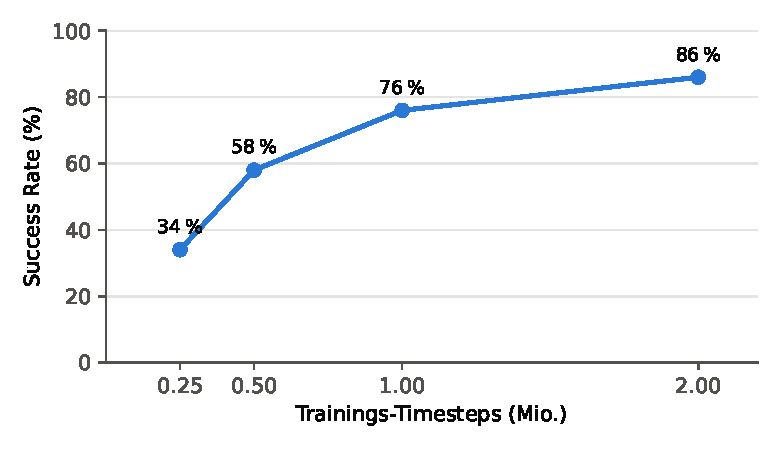
\includegraphics[width=0.72\textwidth]{figures/fig_lernkurve.pdf}
\caption{Lernkurve des besten Modells (\texttt{ppo\_lstm\_curriculum},
Curriculum-Phase 3, stochastische Evaluation auf 50 Seeds).}
\label{fig:lernkurve}
\end{figure}

\subsection{Der Det/Stoch-Gap und die POMDP-These}

Auffällig ist die Lücke zwischen stochastischer (86\,\%) und deterministischer
(36\,\%) Evaluation: Die Argmax-Politik folgt dem Luftlinien-Kompass in konkave
Wandtaschen und oszilliert dort in 2-Schritt-Schleifen; beim Sampling bricht der
Zufall diese Schleifen. Wir interpretieren dies als inhärente Eigenschaft der
POMDP-Struktur (der Kompass zeigt durch Wände) in Kombination mit begrenzter
LSTM-Kapazität --- die stochastische Evaluation ist daher die primäre Metrik,
der Gap wird als Limitation ausgewiesen und gezielt adressiert (Ausblick,
Abschnitt~\ref{sec:ausblick}).

\subsection{Hyperparameter-Fehleranalyse (v7--v10)}

Eine Serie fehlgeschlagener Verbesserungsversuche (v7--v9: Success Rate
$\leq$12\,\%, \texttt{approx\_kl}$\approx$0, \texttt{explained\_variance}$\approx$0)
wurde durch Reverse-Engineering des funktionierenden v2-Modells aufgeklärt:

\begin{table}[h]
\centering
\small
\begin{tabular}{@{}lrrl@{}}
\toprule
\textbf{Parameter} & \textbf{v2 (86\,\%)} & \textbf{v7--v9 (0--12\,\%)} & \textbf{Wirkung des Fehlers} \\
\midrule
\texttt{ent\_coef} & 0.05 & 0.01 & zu wenig Exploration; Exit wird nie gefunden \\
\texttt{n\_steps} & 256 & 512 & BPTT zu lang $\to$ verschwindende Gradienten \\
\texttt{batch\_size} & 8 & 256 & zu wenige Gradient-Updates pro Rollout \\
Obs-Dimension & 231 & 249 & Zusatzfeatures ohne funktionierende Basis \\
\bottomrule
\end{tabular}
\caption{Root-Cause-Analyse: \texttt{ent\_coef} erwies sich als dominanter
Faktor. Die Reproduktion der v2-Konfiguration (v10) stellte das Lernen wieder
her.}
\label{tab:rootcause}
\end{table}

\section{Entwicklungsverlauf: Von der Baseline zum LSTM-Agenten}
\label{sec:entwicklung}

Dieser Abschnitt dokumentiert die Entwicklung des RL-Teils chronologisch von
Projektbeginn bis heute. Primärquelle ist das durchgängig geführte
Experiment-Changelog (\texttt{CHANGELOG.md}), in dem jede Änderung mit Problem,
Lösung und Messergebnis festgehalten wurde. Negative Ergebnisse sind bewusst
enthalten --- sie haben die Architekturentscheidungen maßgeblich geprägt.

\subsection{Etappe 1 (Mai 2026): Baselines mit BFS-Orakel}

Nach Fertigstellung der Spiel-Engine (Mitte Mai) begann das RL-Training mit
Features aus dem BFS-Distanzfeld \emph{in der Observation} (5 Werte: aktuelle
Distanz + 4 Nachbarrichtungen) --- einem \glqq Orakel\grqq, das dem Agenten die
lokal richtige Richtung verriet.

\textbf{Fehlstart mit DQN:} Der erste Agent (DQN) lernte nicht --- Diagnose:
korrupter Replay-Buffer, 2-Zellen-Oszillationen, und eine Visited-Mask in der
Observation (455 Dimensionen), die sich jeden Schritt änderte und den
Q-Wert-Argmax destabilisierte. Konsequenz: Wechsel auf PPO, Visited-Mask
entfernt.

\textbf{BFS-Kraftfeld-Bug:} Ein Oracle-Test (greedy dem BFS-Feld folgen)
scheiterte in 3/3 Seeds --- \texttt{bfsDistanceAt()} lieferte für Wand-Tiles
einen Manhattan-Fallback, wodurch Wände als attraktive Richtung erschienen.
Nach dem Fix (Wand $\to$ 9999): Oracle 3/3. Dieser Test wurde zum
Standard-Werkzeug, um Umgebung und Reward von Trainingsproblemen zu trennen.

\textbf{Curriculum-Lektion:} Phase-1-Training (Exit 5--12) erreichte 56\,\%,
aber der naive Transfer auf Phase 2 (12--25) kollabierte (22\,\% $\to$ 6\,\%)
--- die eingebrannte Kurzdistanz-Politik ließ sich nicht überschreiben.
Lösung: Mixed-Distribution-Training (Exit 5--45). Damit erreichte
\emph{Phase 3} 86\,\% stochastisch auf Testset A (drei unabhängige Läufe:
$85{,}3 \pm 3{,}8\,\%$ auf A, $79{,}3 \pm 8{,}1\,\%$ auf B) und \emph{Phase 4}
nach Reward-Tuning 98\,\% (A) / 94\,\% (B).

\textbf{Der deterministische Kollaps:} Trotz 98\,\% stochastischer SR lag die
Argmax-Auswertung bei 2\,\%. Die Analyse fand die Wurzel in der
Feature-Kodierung: Die BFS-Absolutwerte ($/64$) unterschieden sich zwischen
Nachbarzellen nur um $\approx 0{,}016$ --- zu wenig für eine robuste
Richtungspräferenz, und Wände waren durch Clamping nicht von \glqq weit
weg\grqq{} unterscheidbar (Aliasing). Der Wechsel auf
\emph{Delta-Kodierung} (Richtungssignal $\pm 0{,}5$ statt $0{,}016$, Wand
$= +1{,}0$) hob die deterministische SR auf 42\,\% (offene Welt) bzw.\
100\,\% (wanddichte Hard-World); Temperature-Sampling ($\tau = 0{,}2$)
erreichte 100\,\% bei $\varnothing$ 90 Schritten. Ein Experiment, exitDx/exitDy
zu entfernen (\glqq Phase 5\grqq), scheiterte (max.\ 40\,\%) --- der
Luftlinien-Kompass ist als Fernbereichssignal notwendig.

\subsection{Etappe 2 (Juni 2026): Kernbeitrag --- Navigation ohne Orakel}

Mit funktionierender Baseline wurde die Forschungsfrage geschärft: \emph{Kann
der Agent auch ohne BFS-Orakel in der Observation navigieren?} Der Wechsel auf
RecurrentPPO (LSTM) mit Curriculum, Explorations-Bonus und step\_frac-Feature
(231-dim Obs, kein BFS) lieferte am 08.06.2026 das zentrale Ergebnis:
\textbf{86\,\% stochastisch / 36\,\% deterministisch} auf Testset A und
68\,\% / 18\,\% auf Holdout B --- beide Zielkriterien stochastisch erfüllt,
erstmals ohne Wegweiser-Orakel (Abbildung~\ref{fig:entwicklung},
Ablation in Tabelle~\ref{tab:ablation}). Parallel wurde die POMDP-These
formuliert (Abschnitt~\ref{sec:ablation}) und, inspiriert vom
PokéRL-Projekt, Infrastruktur ergänzt: Seed-Pool (Swarm), WebSocket-Live-Map,
Heatmap-Evaluation, Early-Stop-Truncation.

\begin{figure}[h]
\centering
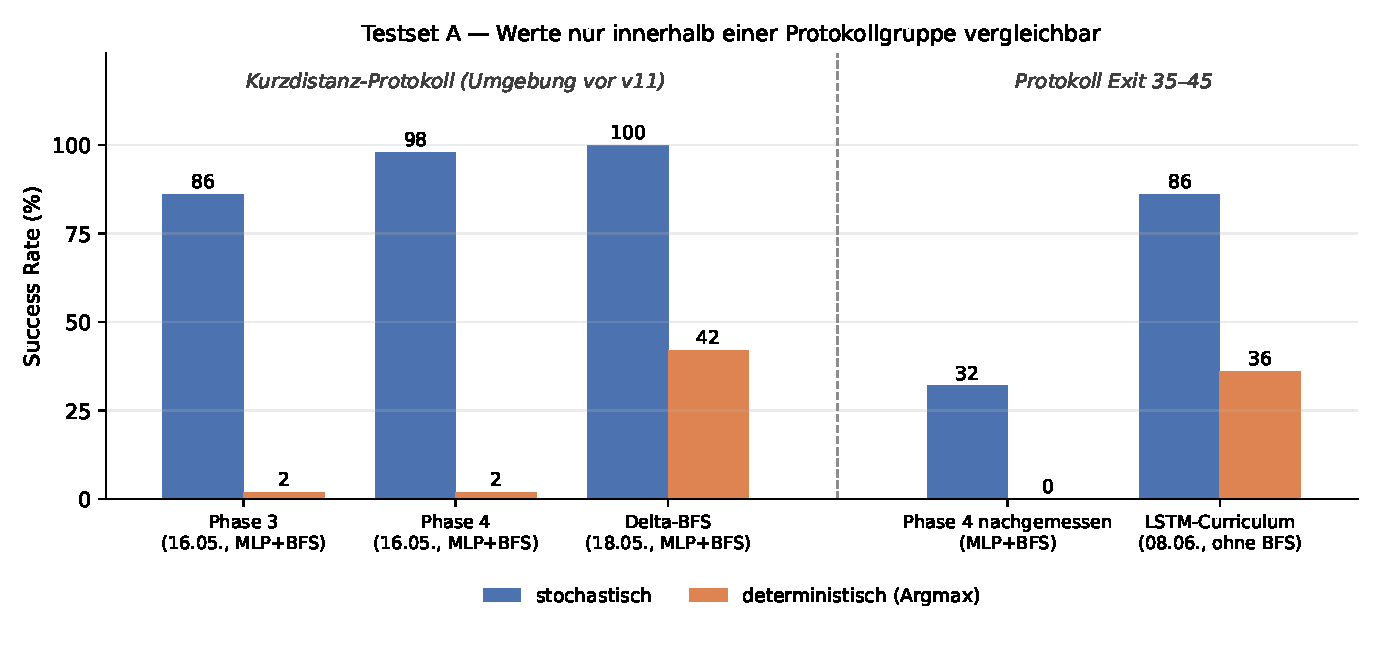
\includegraphics[width=0.85\textwidth]{figures/fig_entwicklung.pdf}
\caption{Entwicklung über die Modellgenerationen (Testset A, Exit 35--45).
Links die MLP-Baselines mit BFS-Orakel in der Observation, rechts der
LSTM-Agent ohne Orakel --- der Kernbeitrag: nahezu gleiche stochastische
Leistung ohne globale Pfadinformation. Der Det/Stoch-Gap zieht sich als
zentrales Thema durch alle Generationen.}
\label{fig:entwicklung}
\end{figure}

\textbf{Methodische Härtung (11.06.):} Ein Data-Leakage-Fehler wurde entdeckt
und behoben --- der Trainings-Callback hatte Modellauswahl und Phasenwechsel
auf den \emph{Test}-Seeds (7000er) gesteuert; seitdem existiert das getrennte
Validierungsset (6000er). Zusätzlich wurde die Lösbarkeit aller relevanten
Welten bewiesen (3\,150 Seeds, 100\,\%).

\subsection{Etappe 3 (13.--25.06.): Hyperparameter-Krise und Root-Cause-Analyse}

Eine Serie von Verbesserungsversuchen (v6--v9: Wand-Penalty-Entfernung,
visit\_count- und Action-Buffer-Features, diverse Batch-/Epochen-Kombinationen)
scheiterte durchgängig (SR 0--12\,\%, \texttt{approx\_kl} $\approx$ 0). Die
Aufklärung gelang durch \emph{Reverse-Engineering} des letzten funktionierenden
Modells (v2): Die zwischenzeitlichen \glqq Optimierungen\grqq{} hatten
unbemerkt die kritischen Hyperparameter verstellt
(Tabelle~\ref{tab:rootcause}); dominanter Faktor war
\texttt{ent\_coef} ($0{,}05 \to 0{,}01$: der Agent explorierte nicht mehr
genug, um den Exit je zu finden). Die v2-Reproduktion (v10) stellte das Lernen
wieder her; der abgeschlossene Lauf vom 25.06.\ erreichte 86\,\% (Validierung)
nach 2{,}2\,Mio.\ Steps in 3\,h\,12\,m --- das aktuelle Referenzmodell
(Abbildung~\ref{fig:lernkurve}).

\subsection{Etappe 4 (06.07.2026): Umgebungsrevision v11 und Performance}

Ein systematisches Audit (Umgebung, Reward, Trainingspipeline, Usability)
führte zu zehn dokumentierten Änderungen --- Details in
Abschnitt~\ref{sec:v11} und Abschnitt~\ref{sec:performance}. Höhepunkte:
präzise Schwierigkeitssteuerung über BFS-Laufweg, Behebung eines
prozess-globalen Config-Lecks (das zuvor unbemerkt die
Phase-3-Trainingsverteilung verschob), Entfernung toter Features und
Straf-Terme, sowie die validierte Verdopplung der Trainingsgeschwindigkeit
(batch\_size 8 $\to$ 64, CPU statt GPU).

\subsection{Etappe 5 (07.07.2026): Erster v11-Gesamtlauf, Monitoring-Redesign
und Seed-Replay-Analyse}
\label{sec:etappe5}

\textbf{Erster v11-Gesamtlauf (Seed 0, laufend).} Der erste vollständige
Curriculum-Lauf auf der revidierten v11-Umgebung
(\texttt{models/ppo\_lstm\_curriculum\_v11}) zeigt ein lehrreiches
Zwischenbild (Abbildung~\ref{fig:v11kurve}): Phase~1 endete am Step-Limit bei
42\,\% (stochastisch) --- deutlich langsamer als die Batch-Validierung
derselben Konfiguration (52\,\% bereits bei 150\,k). Die Diagnose im
Trainingslog: Die Policy-Updates sind durchgehend gesund
(\texttt{approx\_kl}\,$\approx$\,0.03, stabile Entropie), aber die
\texttt{explained\_variance} des Critics verharrt bei $\approx$\,0.1
(Validierungslauf: 0.72) --- der Lauf ist ein Kandidat für
Initialisierungs-Pech und unterstreicht, warum das Protokoll drei Läufe pro
Konfiguration verlangt. Bemerkenswert: Direkt nach dem Wechsel in Phase~2
stieg die SR auf 48\,\% \emph{bei größerer Exit-Distanz} --- die breitere
Aufgabenverteilung wirkt als Regularisierer.

\begin{figure}[h]
\centering
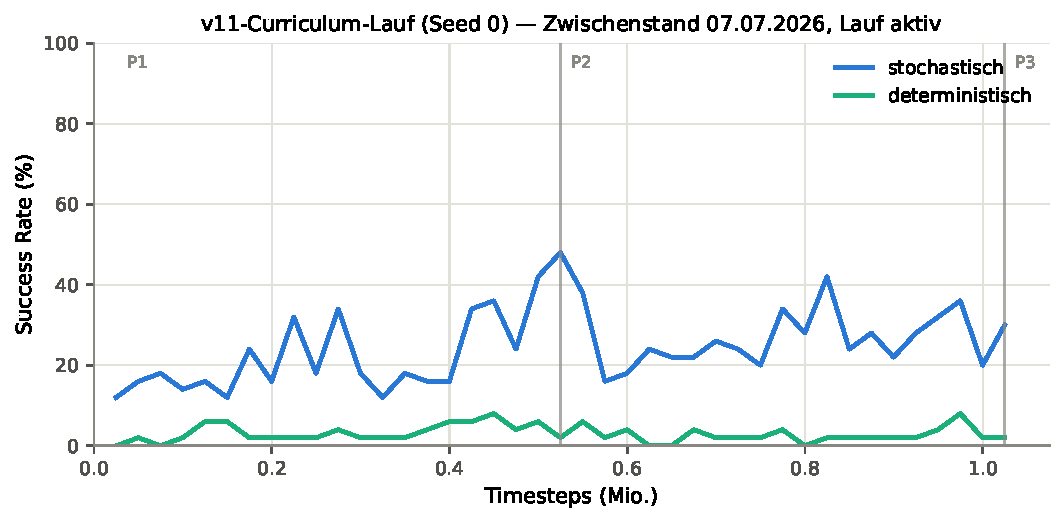
\includegraphics[width=0.85\textwidth]{figures/fig_v11_lernkurve.pdf}
\caption{Lernkurve des ersten v11-Gesamtlaufs (Seed 0, Zwischenstand ---
der Lauf ist zum Redaktionszeitpunkt in Phase 3). Seit v11 misst jeder
Eval-Checkpoint beide Betriebsarten; der Det/Stoch-Gap ist damit erstmals
über den gesamten Verlauf sichtbar. Vertikale Linien: Phasenwechsel
(dort wird jeweils das Bestmodell der Vorphase geladen; die x-Achse ist
über die Phasen kumuliert). Erzeugt mit \texttt{scripts/plot\_run\_curve.py}.}
\label{fig:v11kurve}
\end{figure}

\textbf{Live-Monitoring-Redesign.} Das WebSocket-Dashboard aus Etappe~2 wurde
nach Dashboard- und Farb-Literatur überarbeitet (Abbildung~\ref{fig:livemap}):
(a)~Charts auf uPlot mit EMA-Glättung nach TensorBoard-Vorbild;
(b)~die SR-Kurve zeigt det.\ und stoch.\ getrennt --- der zentrale
Untersuchungsgegenstand war zuvor im Monitoring unsichtbar;
(c)~die Explorations-Heatmap wechselte von der Jet- auf die perzeptuell
uniforme Viridis-Skala (Jet erzeugt künstliche Kontraste und ist nicht
farbfehlsichten-tauglich); (d)~die Agenten-Minimaps rekonstruieren aus dem
gestreamten $15\times15$-Sichtfeld eine wachsende Weltkarte (Wände, Bäume,
Exit) statt nur der Agentenposition. Beim Umbau wurden zwei Fehler gefunden
und behoben: Der Exit-Richtungspfeil war seit der Obs-Umstellung auf 229
Dimensionen stumm defekt, und der SB3-Stepzähler springt beim
Phasenwechsel zurück (es wird das Bestmodell der Vorphase geladen), was
unkorrigiert alle stepbasierten Zeitachsen verfälscht.

\begin{figure}[h]
\centering
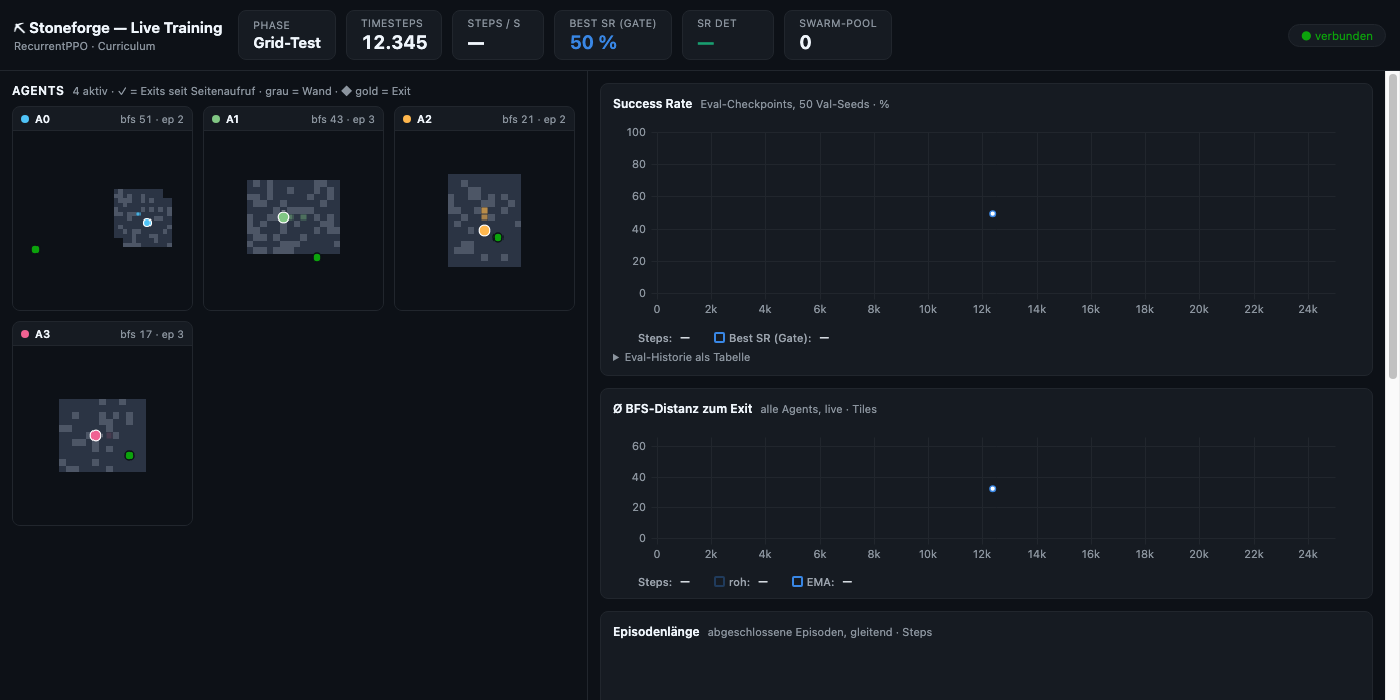
\includegraphics[width=0.9\textwidth]{figures/fig_livemap.png}
\caption{Live-Monitoring (Demo mit Zufallsagenten): KPI-Zeile,
Weltkarten-Minimaps (grau = Wand, blaugrau = erkundeter Boden, grün =
Startpunkt) und uPlot-Charts. Im Training zusätzlich: goldene Raute =
gesichteter Exit, grüner Blitz bei Exit-Erfolg, Viridis-Heatmap.}
\label{fig:livemap}
\end{figure}

\textbf{Seed-Replay-Analyse (Swarm vs.\ PLR).} Das Training wiederholt seit
Etappe~2 bei 30\,\% der Episoden-Resets einen bereits \emph{gelösten} Seed
(\glqq Erfolgs-Swarm\grqq). Ein Literaturabgleich stellt diese Semantik in
Frage: Prioritized Level Replay \cite{jiang2021plr} zeigt, dass das Replay
von Levels mit \emph{hohem Lernpotenzial} --- also gerade \emph{nicht}
gemeisterten --- Sample-Effizienz und Test-Generalisierung verbessert;
das Wiederholen gemeisterter Levels ist der Fehlermodus, den PLR behebt,
und riskiert im Kontext des Projektziels (Generalisierung auf unbekannte
Seeds) Layout-Memorierung. Da der 86\,\%-Referenzlauf jedoch \emph{mit}
Erfolgs-Swarm entstand, wird die Frage nicht per Meinung, sondern als
A/B-Test entschieden (Erfolgs-Swarm vs.\ \texttt{-{}-plr} vs.\
\texttt{-{}-no-swarm}; Maßnahme B8 in \texttt{docs/BEWERTUNG\_UND\_PLAN.md}).
Ein dabei entdeckter Designfehler wurde sofort behoben: Der Seed-Pool
überlebte Phasenwechsel, obwohl ein \glqq gelöster\grqq{} Seed nach dem
Wechsel der Exit-Distanz eine andere Aufgabe beschreibt --- der Pool wird
jetzt bei jedem Phasenstart geleert.

\subsection{Zeitleiste und Lessons Learned}

\begin{table}[h]
\centering
\small
\begin{tabular}{@{}lp{7.6cm}l@{}}
\toprule
\textbf{Datum} & \textbf{Meilenstein} & \textbf{Ergebnis (Testset A)} \\
\midrule
12.05. & Spiel-Engine \& Weltgenerierung spielbar & --- \\
16.05. & DQN-Fehlstart $\to$ PPO; BFS-Kraftfeld-Bug gefixt & Oracle 0/3 $\to$ 3/3 \\
16.05. & Curriculum P1; naiver Transfer kollabiert $\to$ Mixed-Dist. & 56\,\% $\to$ 86\,\% stoch \\
16.05. & Phase 4 (Reward-Tuning), 3-Läufe-Protokoll & 98\,\% stoch / 2\,\% det \\
18.05. & Delta-BFS-Kodierung + Temperature-Sampling & 100\,\% stoch / 42\,\% det \\
07.06. & \textbf{RecurrentPPO ohne BFS-Orakel (Kernbeitrag)} & \textbf{86\,\% / 36\,\%} \\
08.06. & POMDP-These; Callback-Bugs; Swarm/Live-Map & --- \\
11.06. & Data-Leakage behoben (Val-Set 6000er); Lösbarkeit 100\,\% & --- \\
13.--15.06. & v6--v9 scheitern $\to$ Root-Cause (ent\_coef/batch/n\_steps) & 0--12\,\% \\
25.06. & v10-Reproduktion abgeschlossen (Referenzmodell) & 86\,\% (Val) \\
06.07. & Env-Revision v11 (10 Änderungen); batch=64 validiert & 52\,\% stoch @150k (P1) \\
07.07. & Erster v11-Gesamtlauf (Seed 0, läuft); Monitoring-Redesign; Swarm-Analyse (B8) + Pool-Fix & 48\,\% stoch (P2, Val) \\
offen & v11-Lauf abschließen, Seeds 2--3, Swarm-A/B (B8), Det-Gap-Maßnahmen & --- \\
\bottomrule
\end{tabular}
\caption{Zeitleiste der RL-Entwicklung (Auswahl; vollständig in \texttt{CHANGELOG.md}).
SR-Angaben je nach Etappe mit unterschiedlichem Protokoll --- Werte vor dem 11.06.\
ohne strikte Val/Test-Trennung.}
\label{tab:timeline}
\end{table}

\textbf{Lessons Learned (negative Ergebnisse mit Erkenntniswert):}
\begin{itemize}
  \item \emph{Visited-Mask in der Observation} destabilisiert den Argmax
        (jede 1-Bit-Änderung kann die Richtungspräferenz kippen).
  \item \emph{Naiver Curriculum-Transfer} zerstört die Vorgänger-Politik ---
        Mixed-Distribution bzw.\ leistungsbasierte Phasenwechsel sind nötig.
  \item \emph{Feature-Kodierung schlägt Feature-Auswahl:} Der BFS-Gradient war
        nie \glqq zu schwach\grqq{} --- er war falsch kodiert (Delta-Fix: Signal
        $32\times$ stärker).
  \item \emph{Straf-Stacking} (Wand-, Loop-, Stagnations-Penalties) macht
        Stillstand lokal optimal; Information gehört in die Observation, nicht
        in den Reward.
  \item \emph{Hyperparameter dominieren Features:} Alle v7-Feature-Ideen
        scheiterten an verstellten Basis-Hyperparametern; \texttt{ent\_coef}
        war der entscheidende Faktor. Ohne das Changelog wäre die
        Root-Cause-Analyse (v2-Reverse-Engineering) nicht möglich gewesen.
  \item \emph{Eval-Protokoll ist Teil des Experiments:} Data-Leakage über den
        Callback und das Gating auf einer signal-losen Metrik (det.\ SR bei
        hoher Entropie) verzerrten Selektion und Laufzeit unbemerkt.
\end{itemize}

\section{Umgebungsrevision v11 (06.07.2026)}
\label{sec:v11}

Eine systematische Überprüfung der Umgebung gegen Best Practices des
Environment- und Reward-Designs führte zu sieben verifizierten Änderungen:

\begin{enumerate}
  \item \textbf{Tote Features entfernt:} Energie und Inventar waren konstant;
        Observation 231 $\to$ 229 Dimensionen (Tabelle~\ref{tab:obs}).
  \item \textbf{Straf-Stacking entschärft:} Wand-Penalty entfernt, Loop-Penalty
        $-0.15 \to -0.05$ (Tabelle~\ref{tab:reward}).
  \item \textbf{Exit-Platzierung nach BFS-Laufweg:} Zuvor wurden Kandidaten nach
        \emph{Luftlinie} gewählt --- der reale Laufweg bei nominell
        \glqq 35--45\grqq{} streute auf 42--75 Tiles ($\varnothing$ 55). Nach dem
        Fix liegen alle 150 Eval-Seeds exakt im Sollbereich
        (Abbildung~\ref{fig:exitdist}); das Curriculum steuert die Schwierigkeit
        damit erstmals präzise.
  \item \textbf{Prozess-globales Config-Leck behoben:} Die
        Weltgenerierungs-Konfiguration ist im C++-Kern global; parallel
        existierende Umgebungen überschrieben sich gegenseitig (u.\,a.\ verschob
        der Eval-Callback die Phase-3-Trainingsverteilung unbemerkt). Jede
        Umgebung stempelt ihre Konfiguration nun bei jedem Reset neu.
  \item \textbf{Mining/Bauen/Kampf aus dem RL-Pfad entfernt} (Binding erlaubt nur
        noch Aktionen 0--3; tote Reward-Terme gestrichen).
  \item \textbf{Entropie-Annealing korrigiert:} stetig $0.05 \to 0.001$ statt
        Sprung $0.05 \to 0.01$ beim Phasenwechsel.
  \item \textbf{Eval-Callback:} phasengerechtes Gating
        (Tabelle~\ref{tab:curriculum}), Episoden-Caps pro Phase, Det+Stoch-Doppelmessung.
\end{enumerate}

\begin{figure}[h]
\centering
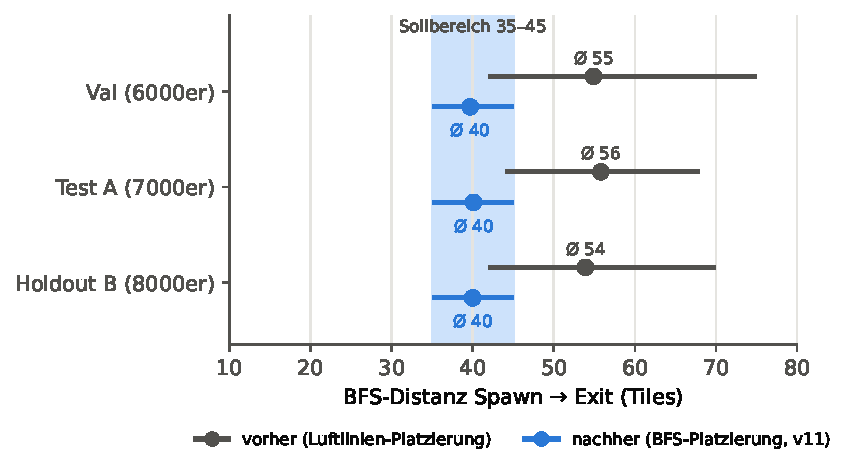
\includegraphics[width=0.8\textwidth]{figures/fig_exit_distanz.pdf}
\caption{Wirkung der BFS-basierten Exit-Platzierung: tatsächliche Laufweg-Distanzen
(min/$\varnothing$/max über je 50 Seeds) vor und nach dem Fix.}
\label{fig:exitdist}
\end{figure}

Alle Änderungen wurden einzeln verifiziert (Lösbarkeit 150/150, Oracle-Agent
10/10 mit exakt BFS-Distanz Schritten, Obs-Layout-Konsistenz, Ablehnung
unzulässiger Aktionen). Da sich die Aufgabenverteilung dadurch ändert, sind
Ergebnisse ab v11 als neue Baseline zu behandeln.

\section{Performance-Analyse: Training beschleunigen}
\label{sec:performance}

\subsection{CPU schlägt Apple-GPU (MPS)}

Ein kontrollierter Benchmark (identisches Trainings-Setup, 8192 Steps) zeigt:
Die GPU ist für dieses kleine Netz (LSTM 256, 229 Inputs) in \emph{jeder}
Konfiguration langsamer als die CPU --- der Kernel-Dispatch-Overhead pro
Mini-Update übersteigt den Rechengewinn (Abbildung~\ref{fig:fps}). Dies deckt
sich mit der Empfehlung der SB3-Autoren, GPUs erst bei CNN-Politiken oder großen
Netzen einzusetzen \cite{raffin2021stable}.

\begin{figure}[h]
\centering
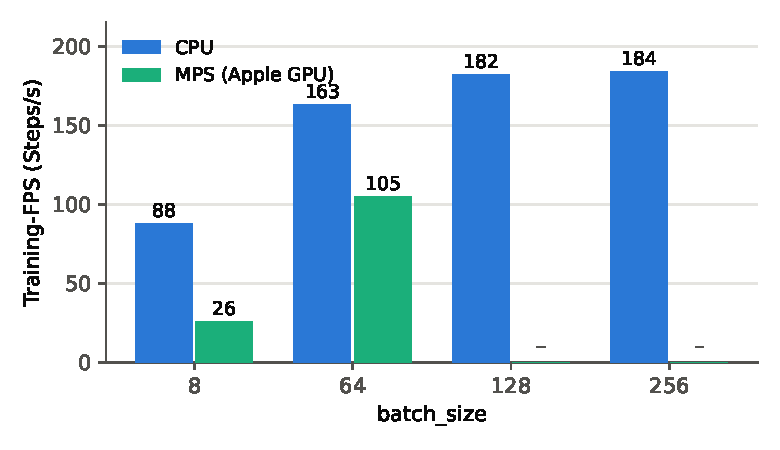
\includegraphics[width=0.72\textwidth]{figures/fig_fps_benchmark.pdf}
\caption{Training-FPS nach Device und Batch-Größe (RecurrentPPO, 16 Umgebungen,
Apple M-Serie). MPS wurde für batch $\geq 128$ nicht weiter gemessen, da bereits
bei 64 unterlegen.}
\label{fig:fps}
\end{figure}

\subsection{Batch-Größe: 2,1-fache Beschleunigung, validiert}

Mit \texttt{batch\_size}=8 fallen pro Rollout 5\,120 Gradient-Updates an ---
mehr Optimizer-Schritte als Umgebungsschritte. Da die Root-Cause-Analyse
(Tabelle~\ref{tab:rootcause}) die Batch-Größe nie isoliert getestet hatte, wurde
ein Validierungslauf durchgeführt: 150k Phase-1-Steps mit \texttt{batch\_size}=64
(Abbildung~\ref{fig:batchval}). Ergebnis: gesunde Lernmetriken
(\texttt{approx\_kl} 0.01--0.06, \texttt{explained\_variance} bis 0.72) und
\textbf{52\,\% stochastische / 22\,\% deterministische SR} nach nur 150k Steps
--- bei \textbf{187 statt 88 FPS}. Die Batch-Größe war demnach \emph{nicht} der
kritische v2-Erfolgsfaktor; \texttt{batch\_size}=64 wurde übernommen
(Gesamtlaufzeit des Curriculums: ca.\ 2,5--3\,h statt 5,5\,h).

\begin{figure}[h]
\centering
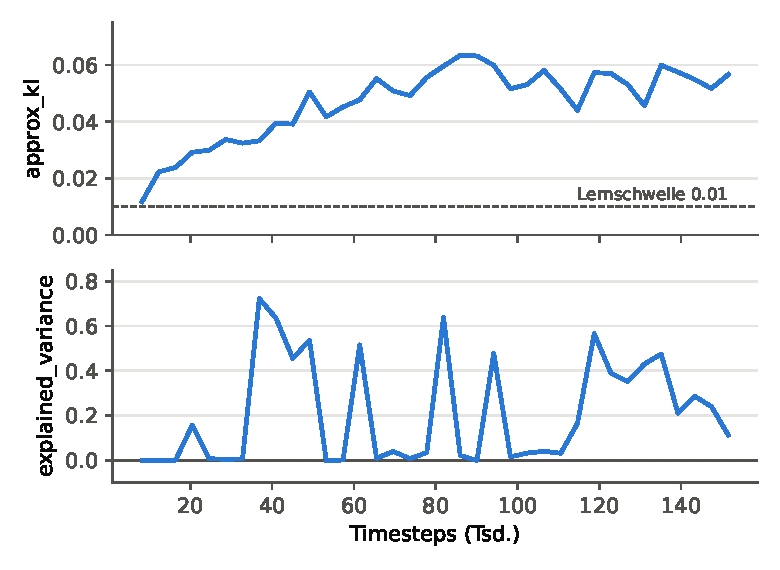
\includegraphics[width=0.72\textwidth]{figures/fig_batch64_validation.pdf}
\caption{Validierungslauf \texttt{batch\_size}=64 (Phase-1-Setup, Env v11):
\texttt{approx\_kl} deutlich über der Lernschwelle, \texttt{explained\_variance}
mit wiederkehrenden Hochphasen --- die Politik lernt aktiv.}
\label{fig:batchval}
\end{figure}

\section{Einordnung in verwandte Arbeiten}

Stoneforge liegt strukturell zwischen drei etablierten Benchmarks: MiniGrid
(teilbeobachtbare Grid-Navigation, PPO+LSTM als Standard-Baseline)
\cite{chevalier2023minigrid}, Crafter (prozedural generiertes 2D-Survival-Spiel
mit Mining und Crafting) \cite{hafner2021crafter} und Procgen (Generalisierung
über prozedurale Level) \cite{cobbe2020procgen}. Publizierte
Zero-Shot-Ergebnisse auf prozeduralen Labyrinthen liegen typischerweise bei
25--53\,\% Success Rate; die hier erreichten 86\,\% (Test) bzw.\ 68\,\%
(Holdout) bei nur 2,2\,Mio.\ Trainingsschritten sind in diesem Kontext ein
starkes Ergebnis. Für die Reduktion des Train/Test-Gaps ist Prioritized Level
Replay \cite{jiang2021plr} der vielversprechendste nächste Baustein; der
vorhandene Seed-Pool-Mechanismus ist eine vereinfachte Variante davon.

\section{Fazit und Ausblick}
\label{sec:ausblick}

\textbf{Stand:} Die Machbarkeit ist gezeigt, beide Zielkriterien sind (stochastisch)
erfüllt, die Umgebung ist nach der v11-Revision methodisch sauber (präzise
Schwierigkeitssteuerung, policy-invariantes Shaping, kein Straf-Stacking, keine
toten Features) und das Training ist doppelt so schnell. \textbf{Offene Schritte:}

\begin{enumerate}
  \item \textbf{v11-Curriculum-Lauf abschließen} (Seed 0 läuft seit 07.07.,
        Abschnitt~\ref{sec:etappe5}); danach Seeds 2--3 für Mittelwert $\pm$
        Standardabweichung.
  \item \textbf{Det/Stoch-Gap schließen:} (a) Temperatur-Sweep der Evaluation
        (wie viel Stochastik braucht die Politik?); (b) Self-Imitation ---
        Nachtraining auf den eigenen erfolgreichen Episoden \cite{oh2018sil},
        um erfolgreiche Trajektorien in die Argmax-Politik zu überführen.
  \item \textbf{Swarm-A/B-Test (B8):} Erfolgs-Swarm vs.\ \texttt{-{}-plr}
        vs.\ \texttt{-{}-no-swarm} --- klärt datenbasiert, ob das
        Erfolgs-Seed-Replay hilft oder der PLR-Semantik \cite{jiang2021plr}
        weichen sollte (Abschnitt~\ref{sec:etappe5}).
  \item \textbf{Falls Holdout B unter Ziel:} vollwertiges Prioritized Level
        Replay (TD-Error-gewichtet) \cite{jiang2021plr}.
\end{enumerate}

\bibliographystyle{unsrt}
\bibliography{references}

\end{document}
